\documentclass[11pt,a4paper]{article}
\usepackage[margin=2.5cm]{geometry}
\usepackage{amsmath,amssymb,booktabs,longtable,tikz,listings,xcolor,hyperref,array}
\usetikzlibrary{arrows.meta,positioning}
\lstset{basicstyle=\ttfamily\footnotesize,breaklines=true,frame=single,columns=fullflexible}
\newcommand{\TODO}[1]{\textcolor{red}{[TO COMPLETE: #1]}}
\title{Development of an Explainable Prolog-Based Expert System for Industrial Chemical Reactor Fault Diagnosis and Corrective Maintenance Planning}
\author{MSc KRR Mini-Project 19}
\date{\today}
\begin{document}\maketitle
\begin{abstract}\TODO{200--300 words written \emph{after} results exist, covering items (i)--(xi) of the brief. Key facts already fixed: jacketed CSTR, 12 fault classes, 18 Horn rules plus abductive and consistency-based reasoning in strictly Prolog, 286 synthetic cases (87 dev / 199 test), explanation facility and maintenance planner.}\end{abstract}
\tableofcontents

\section{Introduction}
\subsection{Engineering context}
A jacketed continuous stirred-tank reactor (CSTR) couples kinetics, heat removal, mixing, pressure and feed quality. A loss of heat removal raises temperature, which raises the Arrhenius rate constant and heat generation, so a thermal excursion can become a runaway \cite{stoessel2008,fogler2016}. Other faults degrade conversion and selectivity, deactivate catalyst or threaten containment. \TODO{8--12 sources for context.}
\subsection{Fault-diagnosis and KRR context}
Detection flags deviation, diagnosis maps symptoms to causes, prognosis predicts progression, and corrective maintenance chooses an action. A knowledge-based system is appropriate where rules, engineering constraints and auditable explanations matter \cite{venkatasubramanian2003}. Diagnosis is treated as deduction ($KB\cup E\models F$), abduction ($D\cup KB\models Obs$) and consistency-based reasoning \cite{reiter1987,dekleer1987} over Horn clauses executed by SLD resolution \cite{lloyd1987,kowalski1974,sterling1994}. Unlike a statistical classifier, every conclusion has a proof.
\subsection{Problem statement, gap, aim}
Heterogeneous, noisy, incomplete and conflicting observations must be mapped to interacting faults with an auditable chain to a maintenance action. \TODO{research-gap table (threshold alarms, model-based, ML, expert systems, KRR) from the literature review.}
\textbf{Aim.} Build and test an explainable Prolog expert system that diagnoses reactor faults and recommends corrective maintenance. \TODO{answer the 12 research questions and 22 objectives in Section 7.}
\subsection{Scope and limitations}
Synthetic steady-state data only; see Section~\ref{sec:lim}. Synthetic values are never presented as plant measurements.

\section{Theoretical Foundation and Knowledge Representation}
\subsection{Reactor, assumptions and operating envelope}
Liquid-phase, first-order exothermic reaction A$\to$products in a perfectly mixed jacketed CSTR at steady state; $V_r=2$\,m$^3$, $\dot m_f\in\{0.7,1.0,1.3\}$\,kg/s (low/nominal/high), $T_r\approx350$\,K held by jacket flow, $\Delta H_r=-150$\,kJ/mol, $E_a=60$\,kJ/mol, $C_{A,in}=2000$\,mol/m$^3$. Under faults the controller output is held (manual/saturated). All parameters are engineering assumptions.
\subsection{Fault taxonomy}
$\mathcal F=\{F_K,F_T,F_H,F_C,F_M,F_Q,F_P,F_J,F_S,F_I,F_R,F_N\}$. $F_U$ is merged into $F_C/F_J$ because it has no independent signature with this sensor set.
\begin{longtable}{p{.6cm}p{3.4cm}p{3.6cm}p{4.2cm}}\toprule Id&Meaning&Causes&Symptoms\\\midrule\endhead
$F_K$&Catalyst degradation&poisoning, sintering&$X\downarrow$, $T\downarrow$, duty$\downarrow$\\
$F_T$&Feed-temperature excursion&pre-heater fault&$T_{in}\uparrow$, $T\uparrow$, $X\uparrow$\\
$F_H$&Heat-transfer loss&jacket fouling&$T\uparrow$, $X\uparrow$; supply, feed, flow normal\\
$F_C$&Cooling fault&chiller/utility&$T_{j,in}\uparrow$, $T_j\uparrow$, $T\uparrow$\\
$F_M$&Mixing fault&drive, impeller&$N_a\downarrow$, $I_m\downarrow$, vibration$\uparrow$\\
$F_Q$&Feed quality&blending, contamination&$C_{A,in}\downarrow$, pH$\downarrow$, $X\downarrow$\\
$F_P$&Abnormal pressure&blocked vent, inerts&$P_r$ above $P_{exp}(T)$\\
$F_J$&Jacket leak/circulation&pump, leak&$P_j\downarrow$, $\dot m_j\downarrow$, $T_j\uparrow$\\
$F_S$&Seal fault&seal wear&level$\downarrow$, $r_P\downarrow$, vibration$\uparrow$\\
$F_I$&Temperature sensor&drift, bias&$T_r\neq T_{out}$\\
$F_R$&Feed-flow control&valve, transmitter&$\dot m_f\neq$ load reference\\
$F_N$&Normal&--&all in band\\\bottomrule\end{longtable}
\subsection{Observation vector and variable dictionary}
Measured: $T_r,T_{in},T_{out},T_{j,in},T_j,P_r,\dot m_f,C_{A,in},C_A,C_B,C_P,Q_r,V_r,N_a,P_j,\dot m_j,\mathrm{pH},V_{RMS},I_m$. Derived by the evidence layer: $e_T,e_P,X,S$, residuals $r_P,r_T,\rho_E$. $c_p$ is specific heat, $C_P$ product concentration; no symbol $C_p$ is used (the brief's Eq.~20 clash). Full dictionary: \texttt{docs/KB\_SPECIFICATION.md}. \TODO{paste as table (Appendix C).}
\subsection{Mathematical formulation}
\paragraph{Material balance and kinetics.}
\begin{align}
\tau&=V_r/\dot V_f\\ \dot V_f&=\dot m_f/\rho\\ \frac{dC_A}{dt}&=\frac{C_{A,in}-C_A}{\tau}-r_A\\ r_A&=aC_A^{\,n},\ n=1\ (\text{rate } k C_A)\\ k&=a\,k_0\exp\!\big(-E_a/(RT_r)\big)\\ X&=\frac{C_{A,in}-C_A}{C_{A,in}}\\ X&=\frac{k\tau}{1+k\tau}\ (\text{steady, first order})\\ S&=\frac{C_P}{C_{A,in}-C_A}\\ C_A+C_B+C_P&=C_{A,in}\ (\text{closure})
\end{align}
\paragraph{Energy balance and heat transfer.}
\begin{align}
\rho V_r c_p\frac{dT_r}{dt}&=\dot m_f c_p(T_{in}-T_r)+(-\Delta H_r)r_AV_r-\dot Q_j\\ \dot Q_{gen}&=\dot Q_r+\dot Q_j\ (\text{steady})\\ \dot Q_{gen}&=(-\Delta H_r)\frac{\dot m_f}{\rho}C_{A,in}X\\ \dot Q_r&=\dot m_f c_p(T_{out}-T_{in})\\ \dot Q_j&=\varepsilon\,\dot m_jc_{pj}(T_r-T_{j,in})\\ \varepsilon&=1-\exp\!\big(-UA/(\dot m_jc_{pj})\big)\\ \dot Q_j&=\dot m_jc_{pj}(T_j-T_{j,in})\ (\text{measured})\\ \Delta T_{lm}&=\frac{\Delta T_1-\Delta T_2}{\ln(\Delta T_1/\Delta T_2)}\\ UA&=\Big[\tfrac1{h_iA_i}+R_f+\tfrac1{h_oA_o}\Big]^{-1}\\ Re&=\frac{\rho vD_h}{\mu}\\ Pr&=\frac{c_p\mu}{k_f}\\ Nu&=\frac{hD_h}{k_f}\\ \rho_E&=\frac{\dot Q_{gen}-\dot Q_r-\dot Q_j}{\dot Q_{gen}}\\ \Delta T_{ad}&=\frac{(-\Delta H_r)C_{A,in}}{\rho c_p}\\ \frac{d\dot Q_{gen}}{dT}&>\frac{d\dot Q_{rem}}{dT}\ (\text{runaway condition})
\end{align}
\paragraph{Mechanical, pressure and leak relations.}
\begin{align}
P_{agit}&=N_p\rho N^3D^5\\ \omega&=2\pi N_a/60\\ \dot W_m&=\tau_m\omega\\ I_m&=I_0+I_1(N_a/N_{a,0})^2\\ P_rV_g&=n_rRT_r\\ P_{exp}&=P_{atm}+P_v(T)\approx101.3+8e^{0.045(T-300)}\\ r_P&=P_r-P_{exp}(T_{best})\\ \frac{dV_r}{dt}&=\dot V_{in}-\dot V_{out}-\dot V_{leak}\\ \dot m_{j,out}&=\dot m_{j,in}-\dot m_{leak}\\ r_T&=|T_r-T_{out}|
\end{align}
\paragraph{Deviation, states and evidence aggregation.}
\begin{align}
d_x&=\frac{x-x_{ref}}{x_{ref}}\\ \epsilon_T&=\frac{T_r-T_{ref}}{T_{ref}},\quad \epsilon_P=\frac{P_r-P_{ref}}{P_{ref}}\\ z_x&=\frac{x-\mu_x}{\sigma_x}\\ \mathrm{state}(x)&=\begin{cases}\text{low}&d_x<\ell_x\\\text{high}&d_x>u_x\\\text{normal}&\text{otherwise}\end{cases}\\ E(F_k)&=\sum_iw_ie_i(F_k)\\ C(F_k)&=E(F_k)/\textstyle\sum_iw_i\\ P(F_k|E)&\propto P(E|F_k)P(F_k)\\ \mathrm{Score}(D)&=\sum_{v\in Ex(D)}w_v+\lambda|R(D)|-\mu|D|
\end{align}
\paragraph{Logic and diagnosis.}
\begin{align}
KB\cup E&\models F\\ D\cup KB&\models Obs\\ KB\cup Obs\cup D&\not\models\bot\\ D^*&=\arg\min_{D}|D|\\ KB\cup Obs\cup D&\models Maint\\ D&\text{ hits every conflict set }CS_j\ (\text{Reiter})
\end{align}
\paragraph{Evaluation.}
\begin{align}
\mathrm{Acc}&=\tfrac{TP+TN}{TP+TN+FP+FN}\\ \mathrm{Prec}&=\tfrac{TP}{TP+FP}\\ \mathrm{Rec}&=\tfrac{TP}{TP+FN}\\ F_1&=\tfrac{2\,\mathrm{Prec}\,\mathrm{Rec}}{\mathrm{Prec}+\mathrm{Rec}}\\ \mathrm{Cov}&=N_{definite}/N_{test}\\ \mathrm{FAR}&=N_{normal\to fault}/N_{normal}\\ \mathrm{ExplRate}&=N_{explained}/N_{diagnosed}\\ \mathrm{PlanValidity}&=N_{valid\,plans}/N_{test}
\end{align}
The set above contains 56 numbered equations (target: $\ge40$); the weights $w$ rank hypotheses only and never decide membership.
\subsection{KRR representation}
Layers: \texttt{state/3} (evidence) $\to$ \texttt{cond/2} (engineering conditions) $\to$ \texttt{r/3} (diagnostic rules). Natural language $\to$ FOL $\to$ Horn $\to$ Prolog, e.g.\ ``a quenched reaction with normal feed quality indicates catalyst degradation'':
\[\forall c:\ \mathit{LowX}(c)\wedge \mathit{LowT}(c)\wedge\neg\mathit{LowFeedConc}(c)\wedge\neg\mathit{LowpH}(c)\rightarrow \mathit{Fault}(c,f_k)\]
\begin{lstlisting}[language=Prolog]
cond(C, activity_loss_pattern) :- cond(C, low_conversion), cond(C, low_reactor_temperature).
r(rk01, fk, C) :- cond(C, activity_loss_pattern), ( observed(C, cain) ; observed(C, ph) ),
                  \+ cond(C, low_feed_concentration), \+ cond(C, low_feed_ph).
\end{lstlisting}
Negation as failure expresses exceptions, but only over \emph{observed} evidence, so missing data never silently counts as ``normal''. Defaults: normal operation unless a primary variable is abnormal; nominal feed assumed when $C_{A,in}$ is unmeasured.
\subsection{Three reasoning modes}
\textbf{Deduction:} \texttt{fired/3} resolves \texttt{r/3} goals by SLD. \textbf{Abduction:} subset-minimal sets of $\le3$ faults whose \texttt{explains/3} effects cover all coverable primary symptoms. \textbf{Consistency:} a hypothesis is rejected when an observed variable contradicts every necessary effect (\texttt{must\_any/2}) or violates \texttt{exclusive/2}. \TODO{one worked formal derivation and one Prolog trace for each mode: generate with \texttt{demos} in \texttt{run\_all}.}

\section{Design and Development of the Prolog Expert System}
\begin{figure}[h]\centering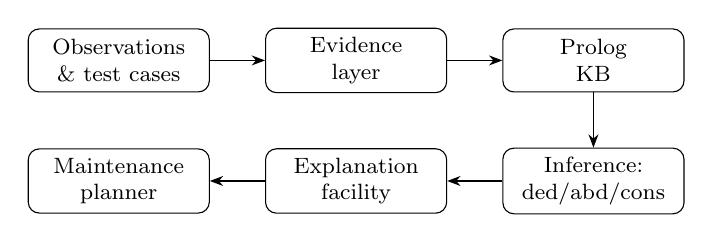
\begin{tikzpicture}[node distance=7mm,box/.style={draw,rounded corners,minimum width=2.3cm,minimum height=8mm,align=center,font=\footnotesize},>=Stealth]
\node[box](o){Observations\\ \& test cases};\node[box,right=of o](e){Evidence\\ layer};\node[box,right=of e](k){Prolog\\ KB};
\node[box,below=of k](i){Inference:\\ ded/abd/cons};\node[box,left=of i](x){Explanation\\ facility};\node[box,left=of x](m){Maintenance\\ planner};
\draw[->](o)--(e);\draw[->](e)--(k);\draw[->](k)--(i);\draw[->](i)--(x);\draw[->](x)--(m);\end{tikzpicture}\caption{Layered architecture (modules: params, evidence, kb, reasoning, explain, planner, eval).}\end{figure}
\subsection{Rule inventory, knowledge acquisition}
18 rules (rk01, rq01--02, rh01, rc01--02, rt01, rj01--02, rm01--03, rs01--02, rp01, rr01--02, ri01); provenance and basis in \texttt{docs/KB\_SPECIFICATION.md} §3. \TODO{extend with the specific papers each rule relies on (literature $\to$ knowledge $\to$ rule $\to$ predicate $\to$ test).}
\subsection{Explanation facility and maintenance planner}
\texttt{explain/1} reports observed evidence, derived conditions, rules fired, diagnosis with evidence confidence, competing/rejected hypotheses and a maintenance plan (fault, evidence, action, urgency, safety constraint, verification). \texttt{sld\_trace/2} prints the proof tree. \TODO{insert one explanation trace from \texttt{results.txt}.}

\section{Dataset, Experimental Methodology and Evaluation}
\subsection{Dataset}
Synthetic only: steady-state model with $\varepsilon$-NTU jacket (Eqs.~7,\,14,\,15), Gaussian sensor noise, fixed seed 20260101, 286 cases: A normal 24, B single 132, C pairs 30, D ambiguous 24, E incomplete 30, F noisy/borderline 31, G sensor+physical 15. Dev/test split 87/199; tolerances tuned on dev only. \textbf{Limitation L1:} generator and KB share the same physics, so results measure internal consistency, not plant performance.
\subsection{Results}
\TODO{paste tables from \texttt{results.txt}: reasoning-mode comparison, per-category results, per-class table, confusion matrix, false-alarm rate, mean/max time, explainability rate, plan validity; ablation (rule groups, evidence classes, tolerance scale, KB growth).}

\section{Software Documentation and Reproducibility}
Environment SWI-Prolog 9.x; commands and layout in \texttt{README.md}; traceability matrix in \texttt{docs/KB\_SPECIFICATION.md} §6. \TODO{record exact SWI version, OS, and final test output.}

\section{Assessment Framework and Deliverables}
\TODO{required tables/figures checklist; contributions; future work (real/plant data, dynamics, more sensors, UI).}

\section{Conclusion}
\TODO{synthesise against research questions after results; must not restate the introduction.}\label{sec:lim}
\paragraph{Limitations to state.} Synthetic and circular data; steady state only; parsimony can mask a weaker fault; sensor-fault detection limited to the $T_r/T_{out}$ pair; $\le3$ simultaneous faults; thresholds are assumptions; maintenance text requires process-safety review.

\begin{thebibliography}{99}\small
\bibitem{fogler2016}Fogler, H. S. (2016). \emph{Elements of chemical reaction engineering} (5th ed.). Prentice Hall.
\bibitem{levenspiel1999}Levenspiel, O. (1999). \emph{Chemical reaction engineering} (3rd ed.). Wiley.
\bibitem{stoessel2008}Stoessel, F. (2008). \emph{Thermal safety of chemical processes}. Wiley-VCH.
\bibitem{seborg2011}Seborg, D. E., Edgar, T. F., Mellichamp, D. A., \& Doyle, F. J. (2011). \emph{Process dynamics and control} (3rd ed.). Wiley.
\bibitem{reiter1987}Reiter, R. (1987). A theory of diagnosis from first principles. \emph{Artificial Intelligence, 32}(1), 57--95.
\bibitem{dekleer1987}de Kleer, J., \& Williams, B. C. (1987). Diagnosing multiple faults. \emph{Artificial Intelligence, 32}(1), 97--130.
\bibitem{venkatasubramanian2003}Venkatasubramanian, V., Rengaswamy, R., Yin, K., \& Kavuri, S. N. (2003). A review of process fault detection and diagnosis: Part I. \emph{Computers \& Chemical Engineering, 27}(3), 293--311.
\bibitem{lloyd1987}Lloyd, J. W. (1987). \emph{Foundations of logic programming} (2nd ed.). Springer.
\bibitem{kowalski1974}Kowalski, R. (1974). Predicate logic as programming language. In \emph{Proceedings of IFIP Congress 74} (pp. 569--574). North-Holland.
\bibitem{sterling1994}Sterling, L., \& Shapiro, E. (1994). \emph{The art of Prolog} (2nd ed.). MIT Press.
\bibitem{poole1989}Poole, D. (1989). Explanation and prediction: An architecture for default and abductive reasoning. \emph{Computational Intelligence, 5}(2), 97--110.
\bibitem{wielemaker2012}Wielemaker, J., Schrijvers, T., Triska, M., \& Lager, T. (2012). SWI-Prolog. \emph{Theory and Practice of Logic Programming, 12}(1--2), 67--96.
\bibitem{incropera2011}Incropera, F. P., DeWitt, D. P., Bergman, T. L., \& Lavine, A. S. (2011). \emph{Fundamentals of heat and mass transfer} (7th ed.). Wiley.
\end{thebibliography}
\TODO{expand to 70--90 unique sources managed in EndNote, APA 7, $\ge60\%$ recent peer-reviewed. This list of 13 is a verified starting set only.}
\end{document}
